\documentclass[conference]{IEEEtran}
\IEEEoverridecommandlockouts

\usepackage{amsmath,amssymb,amsfonts}
\usepackage{algorithmic}
\usepackage{graphicx}
\usepackage{textcomp}
\usepackage{xcolor}
\usepackage[style=numeric]{biblatex}

\addbibresource{references.bib}

\begin{document}

\title{Designing a Controller + Broker}

\author{
\IEEEauthorblockN{Sina Kamali}
\textit{University of Waterloo}\\
\textit{sinakamali@uwaterloo.ca}
}

\maketitle

\section{Introduction}
In this document, we will go over the design details of the controller + broker segment. We will also point out how these two components can be detached if ever needed.

\section{Design}
In this section we will go over the overall design patters used in designing the controller and broker. An overview of the system can be seen in figure~\ref*{fig:odesign}

\begin{figure}[h]
    \centering
    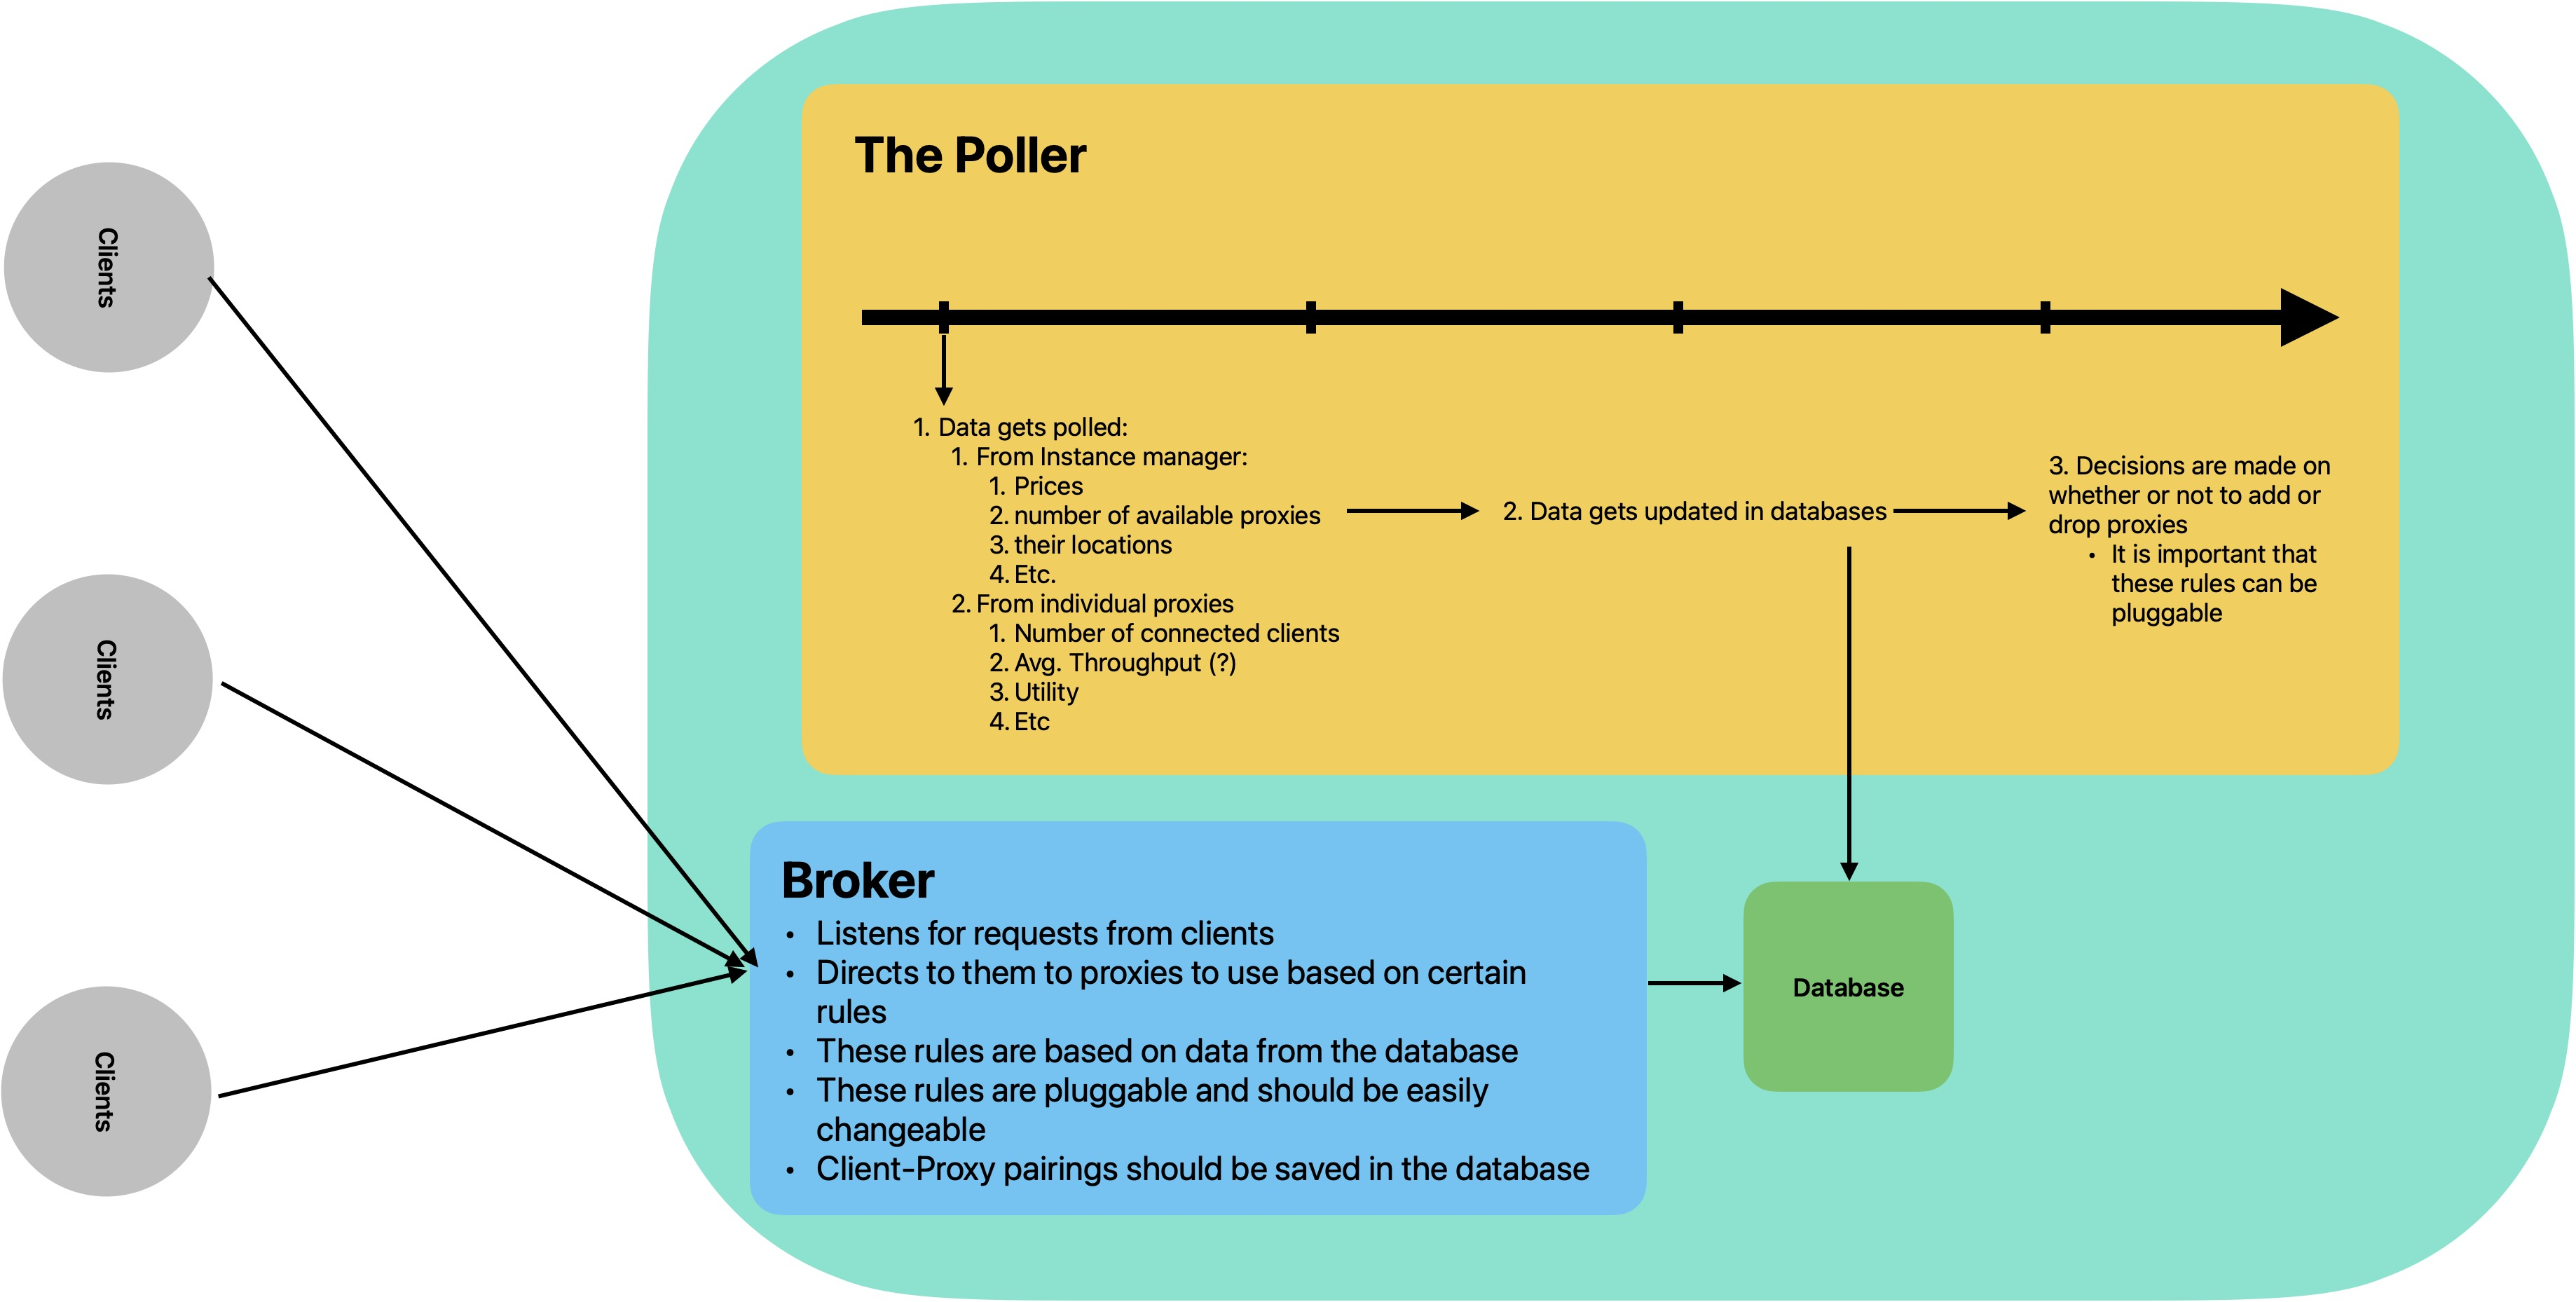
\includegraphics[width=0.4\textwidth]{design.jpeg}
    \caption{overall design}
    \label{fig:odesign}
\end{figure}

\subsection{Designing the Controller}
The controller is in charge of getting information from underlying parties (such as the instance manager and proxies), and updating the database accordingly. The controller gathers these information by periodically polling data endpoints on the proxies and the instance manager. After gathering data, the controller stores them in a database that can be also accessed by the broker. This data will later be used by the broker to assign proxies to clients.

The controller has a database. This database follows a simple relational schema is seen in figure~\ref*{fig:schema}

\begin{figure}[h]
    \centering
    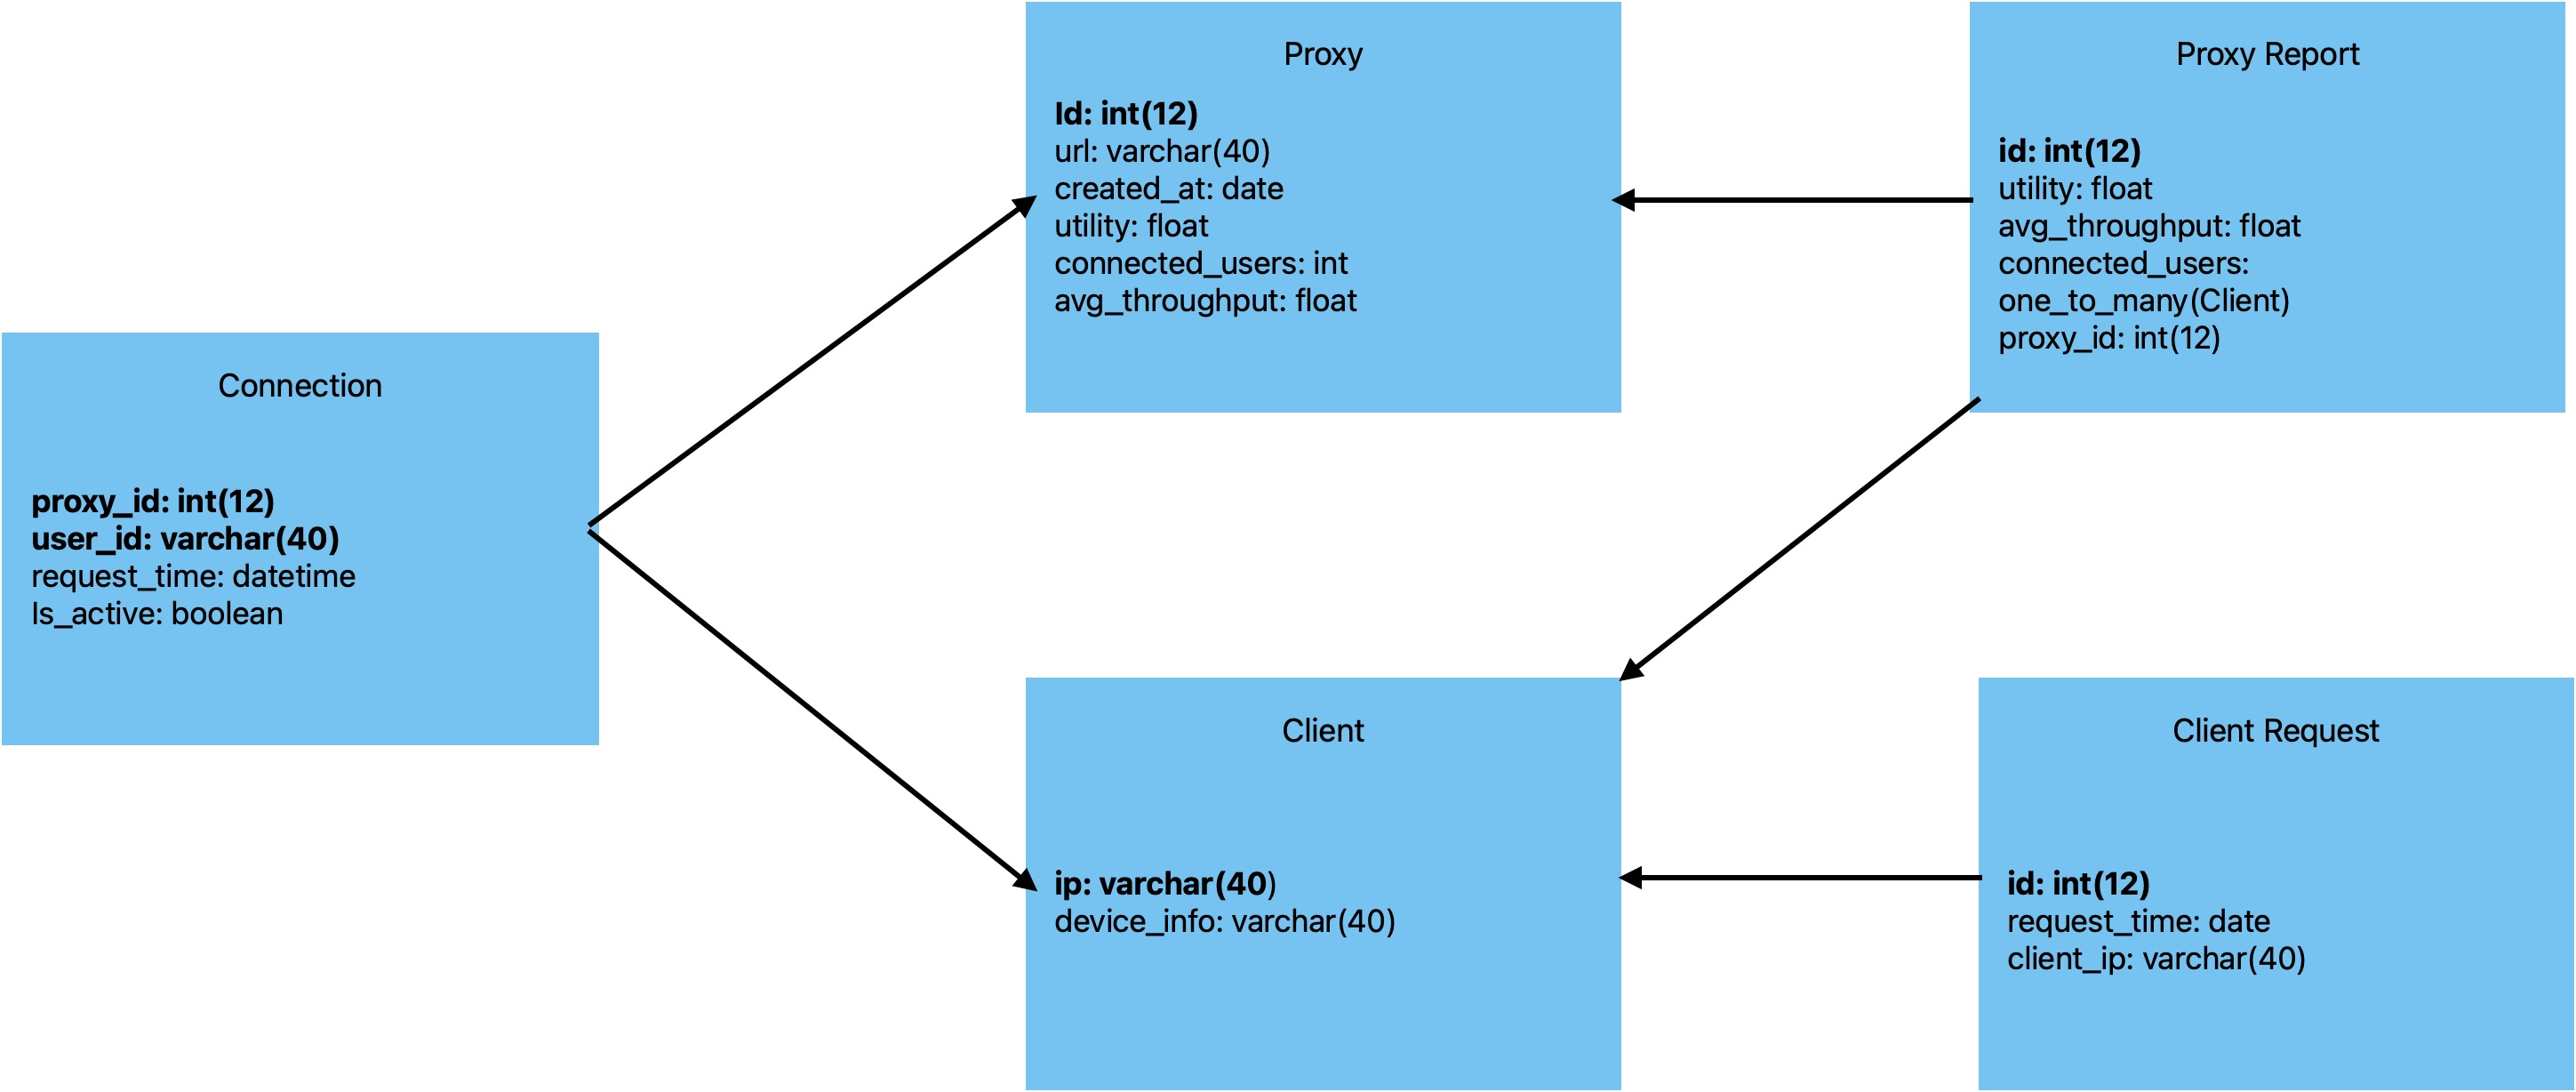
\includegraphics[width=0.4\textwidth]{schema.jpeg}
    \caption{database schema}
    \label{fig:schema}
\end{figure}

\subsection{Designing the Broker}
The broker is the main component that is in charge of assigning proxies to client. Our broker is designed in a way that can easily be integrated with any proxy assignment algorithm.

In this paper we decided to use the proxy assignment algorithm introduced in this \cite{nasr2019enemy} work by Nasr et al. To implement this paper, we used the same formula and attributes they used in their evaluation. All the information needed for the calculation of those features are extracted from the entries in the dataset.

\section{How to decouple the broker and the controller}
To detach the broker and controller systems, one can easily use a third node for a database and then give access to the detached broker and controller systems.

\printbibliography

\end{document}
